\documentclass[10pt]{article}
\usepackage[margin=0.75in]{geometry}
\usepackage{amsmath,amssymb}
\usepackage{tikz}
\setlength{\parindent}{0pt}
\setlength{\parskip}{3pt}
\begin{document}
\title{Precalculus State Competition Problems and Published Solutions}
\date{}
\maketitle
\noindent Each year is grouped separately. The solution beside each problem is the final answer from that year's published answer sheet.
\bigskip
% Precalculus State Packet: 2010-2012
% Each answer below is transcribed from the packet's answer sheet; no worked
% solutions have been added.

\subsection*{State 2010 -- Precalculus}
\begin{enumerate}
\item Let $k$ be selected at random from the set $\{1,2,3,4,6,8,12,18\}$. If $3x=k$, find the probability that the solution for $x$ is a whole number. Express your answer as a common fraction reduced to lowest terms.\\
\textbf{Solution:} $\dfrac12$.

\item Let $x$ be a positive integer such that $x<10$. For how many distinct values of $x$ is $\sin(2x)+1>2$?\\
\textbf{Solution:} $0$ (also accepted: ``Zero'' or ``None'').

\item If the sides of a triangle have lengths $3a$, $2b$, and $c$, with $\angle A$ opposite the side of length $3a$, then
\[
pa^2=qb^2+rc^2-cwb\cos(A).
\]
If $p,q,r,w$ are all positive integers, find the smallest possible value of $p+q+r+w$.\\
\textbf{Solution:} $18$.

\item If $f(x)=3x-4$, then an equation for the inverse can be written as $f^{-1}(x)=\dfrac{x+k}{w}$. Find $k-w$.\\
\textbf{Solution:} $1$.

\item If $x$ is a positive integer, find the smallest possible value of $x$ such that $\cot(x^\circ)$ and $\cot(-x^\circ)$ are equal numbers.\\
\textbf{Solution:} $90$ (degrees optional).

\item From physics, the height $s$, in feet, of an object after $t$ seconds that has been thrown straight up from a point $s_0$ feet above ground level with an initial velocity of $v_0$ is $s=-16t^2+v_0t+s_0$. If a baseball is thrown straight up from 3 feet above ground level with an initial velocity of 97 feet per second, find the number of feet in the maximum height that the ball will reach. Express your answer as a decimal rounded to the nearest hundredth of a foot.\\
\textbf{Solution:} $150.02$.

\item A right circular cylinder has a volume of $12\pi$. The lengths of the radius ($r$) of the base and the height ($h$) of the cylinder are both positive integers. Find the sum of all possible distinct values of $r+h$ where $r$ and $h$ represent the radius and height of one cylinder.\\
\textbf{Solution:} $18$.

\item The probability that Mary will have one of the top ten Precalculus scores is $0.4263$. The probability that Peter will have one of the top ten Precalculus scores is $0.3642$. The probability that both will have scores among the top ten Precalculus scores is $0.1968$. Expressed as a decimal rounded to 4 significant digits, find the probability that both had scores in the top ten Precalculus scores if it is known that at least one of the two did.\\
\textbf{Solution:} $0.3315$.

\item Rounded to the nearest year, find the number of years needed for a sum of money to quadruple if invested at a 7\% annual percentage rate compounded continuously.\\
\textbf{Solution:} $20$ (years optional).

\item In $\triangle ABC$, $AB=7$ and $AC=8$. $\cos(\angle BAC)$ is a rational number that can be expressed as $\dfrac{k}{w}$, where $k$ and $w$ are relatively prime positive integers. It is known that $k+w$ is the square of a positive integer and that $BC$ is a positive integer. Find the sum of all possible distinct values of $BC$.\\
\textbf{Solution:} $14$.

\item A box contains exactly 35 yellow marbles, 7 green marbles, and 8 red marbles. From this box, 5 marbles are drawn (without replacement) at random. Find the probability that the 5 marbles drawn were exactly 3 yellow, 1 green, and 1 red. Express your answer as a common fraction reduced to lowest terms.\\
\textbf{Solution:} $\dfrac{187}{1081}$.

\item \textbf{(Multiple Choice)} For your answer write the capital letter which corresponds to the correct choice. Given: A parabola whose points are all equidistant from the point $(2,5)$ and the line whose equation is $x=7$, and that has a latus rectum of length $16\sqrt5$.
\begin{enumerate}
\item[A)] The conditions above determine a conic.
\item[B)] The conditions above overdetermine a conic (that is, there is no conic meeting all the given conditions).
\item[C)] The conditions above underdetermine a conic (that is, there is more than one conic that meets all the given conditions).
\end{enumerate}
\textit{Note: Be certain to write the correct capital letter as your answer.}\\
\textbf{Solution:} B.

\item On the circle whose equation is $(x-25)^2+(y-30)^2=145$, a particle is at $A(26,42)$ and another particle is at $B(24,18)$. At the same instant, both particles begin to move on the circle. The particle at $A$ moves at a constant speed counterclockwise on the circle, and the particle at $B$ moves at a constant speed clockwise on the circle. The two particles meet for the first time at $(17,39)$. The particle that started at $A$ is moving $k$ times the rate of the particle that started at $B$. Find $k$. Express your answer as a decimal rounded to the nearest hundredth.\\
\textbf{Solution:} $0.35$.

\item In this problem, assume that the standard deviation is calculated according to the standard method of calculating the standard deviation for a set of sample proportions. Also, assume the following table of $z$-scores with the accompanying standard normal probabilities is accurate. On the table, $-2(.0228)$ means there is a normal probability of $.0228$ of obtaining a $z$-score of $-2$ or less.
\[
\begin{array}{rrrrr}
-2(.0228)&-1.9(.0287)&-1.8(.0359)&-1.7(.044)&-1.6(.054)\\
-1.5(.0668)&-1.45(.0735)&-1.4(.0808)&-1.35(.085)&-1.3(.0968)\\
-1.25(.1056)&-1.2(.1151)&-1.1(.1357)&-1(.1587)&-0.9(.1841)\\
-0.8(.2119)&-0.75(.2266)&-0.7(.2420)&-0.6(.2743)&-0.5(.3085)\\
-0.4(.3446)&-0.3(.3821)&-0.25(.4013)&-0.1(.4602)&0(.5000)\\
0.1(.5398)&0.2(.5793)&0.25(.5987)&0.3(.6179)&0.4(.6554)\\
0.5(.6915)&0.6(.7257)&0.7(.7580)&0.75(.7734)&0.8(.7881)\\
0.9(.8159)&1.0(.8413)&1.1(.8643)&1.2(.8849)&1.25(.8944)\\
1.3(.9032)&1.4(.9192)&1.5(.9332)&1.6(.9452)&1.7(.9554)\\
1.75(.9599)&1.8(.9641)&1.9(.9713)&2.0(.9772)&2.1(.9821)\\
2.2(.9861)&2.25(.9878)&2.3(.9893)&2.4(.9918)&2.5(.9938)
\end{array}
\]
Assume that 80\% of all athletes know the value of $\sqrt3$ to 4 significant digits. In a sample observation, Carol selects 100 athletes at random. Find the probability that the proportion of those athletes who know the value of $\sqrt3$ to 4 significant digits is between 76\% and 82\%. Express your answer as a decimal rounded to 4 decimal places.\\
\textbf{Solution:} $0.5328$.

\item Let $a,b,c$ be positive integers. Find all ordered triples $(a,b,c)$ such that
\[
\begin{bmatrix}3&4&7\\2&1&8\end{bmatrix}
\begin{bmatrix}a\\b\\c\end{bmatrix}
=\begin{bmatrix}148\\157\end{bmatrix}.
\]
Be certain to express your answer as ordered triples of the form $(a,b,c)$.\\
\textbf{Solution:} $(1,3,19)$ and $(6,1,18)$, in either order.

\item If $x^4-15x^2+36$ is factored over the reals into four linear factors, one of those linear factors, in simplest form, is $x-k\sqrt{w}$, where $k$ and $w$ are positive integers greater than one. Find $5k+3w$.\\
\textbf{Solution:} $19$.

\item If a stick is broken at random into 3 pieces, find the probability that the longest of the 3 pieces is at least three times the shortest of the 3 pieces and that the 3 pieces can serve as the 3 sides of a triangle. Express your answer as a common fraction reduced to lowest terms.\\
\textbf{Solution:} $\dfrac1{14}$.

\item If $f(x)=\begin{cases}x-2&\text{if }x\leq 0,\\x^2+1&\text{if }x>0,\end{cases}$ then the range of $f$ can be expressed in interval notation as $(-\infty,k]\cup(w,\infty)$. Find $2k+11w$.\\
\textbf{Solution:} $7$.

\item The coordinate axes of the graph of the equation $7x^2+8\sqrt6\,xy-5y^2=28$ are rotated through a positive acute angle ($\theta$) so as to eliminate the $xy$ term. Find $\sin(\theta)$. Express your answer as a decimal rounded to the nearest ten-thousandth.\\
\textbf{Solution:} $0.488$.

\item In the figure shown, $AB=AC=15$, $BD=3$, and $DC=19$. Points $A,E,$ and $B$ are collinear; points $B,D,$ and $C$ are collinear; and points $A,F,$ and $C$ are collinear. $AE=DE$, and $AF=DF$. Find $DE$. Express your answer as a decimal rounded to the nearest hundredth.\\
\textbf{Solution:} No solution.
\end{enumerate}
% 2011 Precalculus State Packet (problems and printed answers)
% The diagrams use TikZ; include \usepackage{tikz} in the document preamble.
\subsection*{State 2011 -- Precalculus}
\begin{enumerate}
\item Let $i=\sqrt{-1}$. If $k$ and $w$ are real numbers such that
\[
  \frac{k+wi}{10-24i}=5,
\]
find the value of $k+w$. \(\text{Solution: }-70\)

\item Let $k$ be a real number. Find the value of
$\sin^2(3567894k)+\cos^2(3567894k)$. \(\text{Solution: }1\)

\item Find the value of the indicated sum:
\[
  \sum_{k=1}^{4}(2k+3).
\]
\(\text{Solution: }32\)

\item Find the sum of the terms of an infinite geometric sequence whose first four terms are $2$, $-1$, $\frac12$, and $-\frac14$. Express your answer as an improper fraction reduced to lowest terms. \(\text{Solution: }\frac43\)

\item In the diagram, points $A$, $B$, and $C$ are collinear. If $\angle DBA=17.13^\circ$ and $\angle DCA=11.87^\circ$, and $DA=967.3$, find $BC$. Round your answer to the nearest integer and express your answer as that integer.
\[
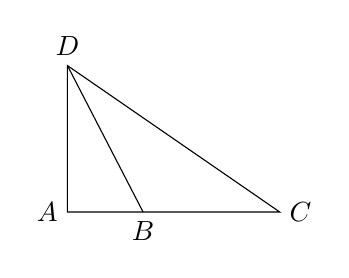
\begin{tikzpicture}[scale=0.62,baseline=(current bounding box.center)]
  \coordinate (A) at (0,0);
  \coordinate (B) at (1.55,0);
  \coordinate (C) at (4.35,0);
  \coordinate (D) at (0,3.0);
  \draw (D)--(A)--(C)--cycle;
  \draw (D)--(B);
  \node[left] at (A) {$A$};
  \node[below] at (B) {$B$};
  \node[right] at (C) {$C$};
  \node[above] at (D) {$D$};
\end{tikzpicture}
\]
\(\text{Solution: }1464\)

\item Let $\vec a$, $\vec b$, $\vec c$, and $\vec d$ represent vectors such that
$\vec a=(3,2)$, $\vec b=(-8,13)$, and $\vec c=(19,-86)$. Find the ordered pair representing $\vec d$ if $\vec a-\vec b=\vec c+\vec d$. \(\text{Solution: }(-8,75)\)

\item When the sum of the first $k$ terms of the series
$1^2+2^2+3^2+\cdots+n^2+\cdots$ is subtracted from the sum of the first $k$ terms of the series
$1(2)+2(3)+3(4)+\cdots+n(n+1)+\cdots$, the result is $528$. Find the value of $k$. \(\text{Solution: }32\)

\item For the equation $x^2+11x+k=0$, the square of the difference between the roots for $x$ is $120$ more than the sum of the squares of these roots for $x$. Find the value of $k$ for which this is true. \(\text{Solution: }-60\)

\item In the diagram, $\overline{AC}$ and $\overline{EC}$ are common external tangents of the two circles, with points of tangency at $A$, $B$, $D$, and $E$. The circles are tangent at $F$ and have radii of lengths $3$ and $8$. Then
$\sin\angle BCD=\dfrac{k\sqrt{w}}{f}$, where $k$, $w$, and $f$ are positive integers. Find the smallest possible value of $k+w+f$.
\[
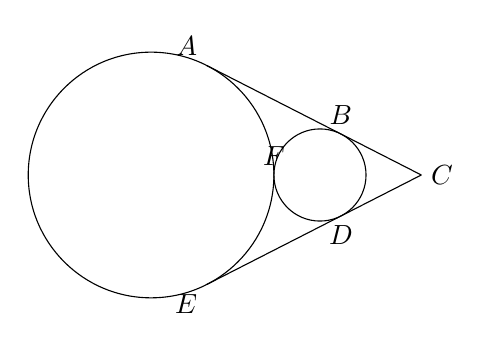
\begin{tikzpicture}[scale=0.78,baseline=(current bounding box.center)]
  \def\R{2.0}
  \def\r{0.75}
  \def\d{2.75}
  \pgfmathsetmacro{\nx}{5/11}
  \pgfmathsetmacro{\ny}{4*sqrt(6)/11}
  \coordinate (O) at (0,0);
  \coordinate (P) at (\d,0);
  \coordinate (A) at ({\R*\nx},{\R*\ny});
  \coordinate (B) at ({\d+\r*\nx},{\r*\ny});
  \coordinate (E) at ({\R*\nx},{-\R*\ny});
  \coordinate (D) at ({\d+\r*\nx},{-\r*\ny});
  \coordinate (C) at ({\R*\d/(\R-\r)},0);
  \coordinate (F) at (\R,0);
  \draw (O) circle (\R);
  \draw (P) circle (\r);
  \draw (A)--(C);
  \draw (E)--(C);
  \node[above left] at (A) {$A$};
  \node[above] at (B) {$B$};
  \node[below] at (D) {$D$};
  \node[below left] at (E) {$E$};
  \node[right] at (C) {$C$};
  \node[above] at (F) {$F$};
\end{tikzpicture}
\]
\(\text{Solution: }167\)

\item Let $x$ represent the degree measure of an angle such that $\cot(x)=\sqrt{3}$. If $180^\circ<x<270^\circ$, find the value of $x$. \(\text{Solution: }210\)

\item Urn A contains five marbles, three of which are orange and two of which are blue. Urn B contains four marbles, three of which are orange and one of which is blue. One of the urns is selected at random, and a marble is then selected at random from that urn. If the marble selected was orange, find the probability that the marble came from Urn B. Express your answer as a common fraction reduced to lowest terms. \(\text{Solution: }\frac59\)

\item A parabola has its line of symmetry parallel to the $x$-axis and has its vertex at $(7,2)$. The point $(3,-8)$ lies on the parabola. Find only the $x$-coordinate of the focus of this parabola. Express your answer as a decimal. \(\text{Solution: }0.75\)

\item Let $\overline{AB}$, $\overline{CD}$, and $\overline{EF}$ be three parallel chords that are non-diameters of a circle on the same side of the center. Let $\overline{GJ}$ be tangent to the circle at $H$ such that $\overline{GJ}\parallel\overline{AB}$. The distance between $\overline{AB}$ and $\overline{CD}$ is equal to the distance between $\overline{CD}$ and $\overline{EF}$ and is also equal to the distance between $\overline{EF}$ and $\overline{GJ}$. If $AB=24$, then $CD$ must be greater than $k$. Find the largest possible simplified exact value of $k$. \(\text{Solution: }8\sqrt6\)

\item A geometric sequence consists of $10$ terms. The sum of the $10$ terms is $2343.7496$, and the sum of the reciprocals of each of the $10$ terms is $1302.0832$. Find the product of the $10$ terms of the original sequence. Express your answer as an exact decimal. \(\text{Solution: }18.89568\)

\item Let $k$ represent a positive integer degree measure such that
$\dfrac{\sin(57^\circ)}{\cos(k^\circ)}=1$. If $0^\circ<k<90^\circ$, find the value of $k$. \(\text{Solution: }33\)

\item The sum of the last two terms of an eight-term geometric progression of real terms is $\frac29$. The sum of the third and fourth terms of this geometric progression is $18$. Find the sum of all eight terms of this geometric progression. Express your answer as an improper fraction reduced to lowest terms. \(\text{Solution: }\frac{1640}{9}\)

\item In rhombus $ABCD$, $\angle DAB=52^\circ$. A circle passes through vertices $A$, $B$, and $D$, and intersects diagonal $\overline{AC}$ at $E$. $CE=12$. Find the length of the arc of the circle from $A$ to $D$ to $B$. Express your answer as a decimal rounded to the nearest hundredth. \(\text{Solution: }39.46\)

\item Let $C(n,k)=\dfrac{n!}{k!(n-k)!}$, where $n$ and $k$ represent positive integers. Find the value of $n$ such that $C(n,5)=792$. \(\text{Solution: }12\)

\item When $(2x+3y)^5$ is expanded and completely simplified, the coefficient of one of the terms is $1080$. Find the exponent of $x$ for that term. \(\text{Solution: }2\)

\item By substituting $1$, $2$, $3$, $4$, $5$, and $6$ for $x$ into a polynomial expression with integral coefficients in $x$, the values are respectively $-3$, $10$, $49$, $120$, $229$, and $382$. If $P(x)$ is the polynomial expression with integer coefficients of lowest degree satisfying the given conditions, find $P(43)$. \(\text{Solution: }91809\)
\end{enumerate}
% 2012 Precalculus State Packet
% Source questions: packet pages 9--11; written answers: page 12.
\subsection*{State 2012 -- Precalculus}
\begin{enumerate}
\item Given the sequence \(1,4,7,10,\ldots,(3n-2)\), if one of the first ten numbers in this sequence is selected at random, find the probability that the number selected is odd. Express your answer as a common fraction reduced to lowest terms. \quad\textbf{Solution:} \(\frac{1}{2}\)

\item \textbf{(Multiple Choice)} For your answer, write the capital letter that corresponds to the best answer. For all real \(x\),
\[
\sin\bigl((-810+x)^\circ\bigr)=
\]
\(\mathrm{A})\ \sin(x^\circ)\qquad
\mathrm{B})\ \cos(x^\circ)\qquad
\mathrm{C})\ -\sin(x^\circ)\qquad
\mathrm{D})\ -\cos(x^\circ)\qquad
\mathrm{E})\ \sin\bigl((90+x)^\circ\bigr)\).
Be certain to write the correct capital letter as your answer. \quad\textbf{Solution:} \(\mathrm{D}\)

\item Find the sum of all distinct values of \(x\) such that \(\lvert x-7\rvert=\lvert 2x+1\rvert\). \quad\textbf{Solution:} \(-6\)

\item \textbf{(Multiple Choice)} For your answer, write the capital letter that corresponds to the best answer. Let \(a\) and \(b\) be real numbers, let \(i=\sqrt{-1}\), and let \(\overline{a+bi}\) be the complex conjugate of \(a+bi\). If
\[
(a+bi)\overline{(a+bi)}=33
\]
is graphed in a complex plane, then the graph will be:
\(\mathrm{A})\) A parabola; \(\mathrm{B})\) A circle; \(\mathrm{C})\) An ellipse that is not a circle; \(\mathrm{D})\) A straight line; \(\mathrm{E})\) A hyperbola. Be certain to write the correct capital letter as your answer. \quad\textbf{Solution:} \(\mathrm{B}\)

\item Let \(f=\{((4,3),6),((7,8),9)\}\). Find the sum of all distinct members of the range of \(f\). \quad\textbf{Solution:} \(15\)

\item Find the number of years it will take for a sum of money to double if invested at an annual percentage rate of \(8.1\%\) and compounded continuously. Express your answer as a decimal rounded to the nearest hundredth of a year. \quad\textbf{Solution:} \(8.56\)

\item If
\[
\begin{bmatrix}3&4\\2&-1\end{bmatrix}
\begin{bmatrix}a&b\\c&d\end{bmatrix}
=
\begin{bmatrix}7&55\\12&22\end{bmatrix},
\]
find the value of \(a+2b+3c+4d\). \quad\textbf{Solution:} \(41\)

\item A person writes down \(5\) different integers at random from the \(25\) integers from \(1\) to \(25\), inclusive. Each of the \(25\) integers is then called off one at a time in a random order. As soon as all \(5\) of the person's numbers have been called off, the person yells, “Bingo.” Exactly how many of the \(25\) numbers will have been called off when the probability that the person will yell “Bingo” for the first time is greatest? \quad\textbf{Solution:} \(25\)

\item Find the exact sum of \(\displaystyle\sum_{w=1}^{9}(-10)^{w-3}\). Express your answer as a decimal. \quad\textbf{Solution:} \(909090.91\)

\item An apartment rental company has \(300\) apartments available, and \(190\) are presently rented at \(\$950\) per month. The company has decided that it will only raise or lower the rent per month on all apartments by integral increments of \(\$40\). A survey has shown that, so long as there are apartments available, for each \(\$40\) drop in rent per month for every apartment, there will be \(99\) new tenants. Find the number of dollars in the monthly rent that will maximize total income. \quad\textbf{Solution:} \(\$870\)

\item In a room with exactly \(6\) distinct persons, exactly \(12\) handshakes between \(2\) distinct persons are made. No two of these handshakes take place between the same \(2\) persons. Of the persons in the room, exactly two persons shook hands with exactly three other persons. Three distinct persons from these \(6\) persons are selected at random. Find the probability that these three distinct persons had all shaken hands with each other from among the \(12\) handshakes. Express your answer as a common fraction reduced to lowest terms. \quad\textbf{Solution:} \(\frac{1}{2}\)

\item Find the number of distinct negative values of \(x\) for which
\[
x^9+2x^7=x^4-7x^3-6x^2-7x+9.
\]
\quad\textbf{Solution:} \(0\)

\item The roots for \(x\) of the equation
\[
x^5-\frac{121}{162}x^4+bx^3+cx^2+dx+e=0
\]
form a geometric progression. The sum of the reciprocals of the roots is \(242\). Find the absolute value of \(e\). Express your answer as a common fraction reduced to lowest terms. \quad\textbf{Solution:} \(\frac{1}{189568}\)

\item An arithmetic progression has a first term of \(3\), and its last term is \(33\). The total population standard deviation \((\sigma_x)\) of the terms of this arithmetic progression is \(\sqrt{105}\). Find the sum of the terms of this arithmetic progression. \quad\textbf{Solution:} \(108\)

\item On April 1, April puts \(1\) cent in her piggy bank, which was empty. On April 2, April puts \(2\) additional cents in her piggy bank. On April 3, April puts \(4\) additional cents in her piggy bank. On April 4, April puts \(8\) additional cents in her piggy bank. She continues this process of doubling the number of cents from the previous day. How many cents will April have in her piggy bank after her deposit on the last day of this April month? \quad\textbf{Solution:} \(1073741823\)

\item In cis form, the roots of \(1-x^5=0\) can be presented as \(\operatorname{cis}(k^\circ)\), where \(k<360\). Find the largest possible value of \(k\). (Note: \(r\operatorname{cis}(\theta^\circ)=r(\cos(\theta^\circ)+i\sin(\theta^\circ))\).) \quad\textbf{Solution:} \(288\)

\item If a stick is broken at random into \(3\) pieces, find the probability that the longest of the \(3\) pieces is at least three times the shortest of the \(3\) pieces. Express your answer as a common fraction reduced to lowest terms. \quad\textbf{Solution:} \(\frac{27}{35}\)

\item Find the radian period of the graph of \(y=3\sin(2x)\). \quad\textbf{Solution:} \(\pi\)

\item The lengths of the sides of a triangle with an area greater than \(4\) are respectively \(13\), \(15\), and \(x\). If \(x\) is a positive integer, find the sum of all distinct possible values of \(x\) such that the cosine of the angle opposite the side of length \(x\) is a positive common fraction with a denominator less than \(37\) when reduced to lowest terms. \quad\textbf{Solution:} \(71\)

\item Observe that
\[
\begin{aligned}
1^3+(-1)^3+0^3&=0^3,\\
2^3+1^3+(-1)^3&=2^3,\\
9^3+15^3+12^3&=18^3,\\
28^3+53^3+75^3&=84^3,\\
65^3+127^3+248^3&=260^3,\\
126^3+249^3+615^3&=630^3.
\end{aligned}
\]
Should this pattern continue, then the next term would be
\[
k^3+w^3+p^3=1302^3.
\]
Find the value of \(k+w+p\). \quad\textbf{Solution:} \(192\)
\end{enumerate}

\subsection*{State 2013 -- Precalculus}
\begin{enumerate}
\item Find the fifth term of an arithmetic sequence whose first and second terms are respectively $1$ and $12$. \textbf{Solution:} $45$.
\item If $f(x)=x^2+5$ and $g(x)=(x+5)^2$, find the value of $f(3)+g(4)$. \textbf{Solution:} $95$.
\item Let $i=\sqrt{-1}$. Find the value of $|7+4i|$. \textbf{Solution:} $\sqrt{65}$.
\item Let $\|(k,w)\|$ represent the norm of the vector represented by $(k,w)$. If $\|(k,9)\|=9\sqrt{5}$ and $k<0$, find $k$. \textbf{Solution:} $-18$.
\item The degree measures of the three angles of $\triangle ABC$ are in the ratio $2:2:5$. The degree measures of the three angles of $\triangle DEF$ are in the ratio $5:11:14$. One of the six angles from these triangles is selected at random. Find the probability that the selected angle has a degree measure of $40$. Express your answer as a common fraction reduced to lowest terms. \textbf{Solution:} $\frac{1}{3}$.
\item The first term of a geometric sequence of real terms is $2$, and the fifth term of this sequence is $18$. If the fourth term of this sequence is negative, find the value of the fourth term. \textbf{Solution:} $-6\sqrt{3}$.
\item Consider the sequence $\{x_n\}$ defined as $x_{n+1}=\frac{6x_n}{7}+\frac{5491}{7x_n}$ for integral $n\geq 1$, and for which $x_1=11$. As $n$ increases without bound, the limiting value of $x_n$ is $k$. Find $k$. \textbf{Solution:} $17\sqrt{19}$.
\item The polynomial equation $x^3+kx^2+wx+p=0$, with $k,w,p$ integers, has $5$ and $1+i$ as two of its roots. If $i=\sqrt{-1}$, find $p$. \textbf{Solution:} $-10$.
\item A plane contains points with coordinates $A(2,-1,1)$, $B(0,-3,0)$, and $C(-1,-2,1)$. A fourth point not on this plane has coordinates $D(5,2,4)$. Find the volume of a tetrahedron with vertices at $A,B,C,$ and $D$. \textbf{Solution:} $1$.
\item If $\frac{(x+k)!}{x!}-x=1$ for all possible values of $x$ where $x$ and $k$ represent positive integers, find $k$. \textbf{Solution:} $1$.
\item Find the sum of the terms of an infinite geometric sequence whose first four terms are $1,-\frac14,\frac1{16},-\frac1{64},\ldots$. Express your answer as a common fraction reduced to lowest terms. \textbf{Solution:} $\frac45$.
\item In a 3-dimensional rectangular coordinate system, the points are $A(1,4,3)$, $B(2,6,8)$, and $C(k,w,f)$. If $\overline{AB}\perp\overline{AC}$, find $k+2w+5f$. \textbf{Solution:} $24$.
\item Team A plays Team B six times in a season. For each game, the probability that Team A will win is $\frac35$. Find the probability that Team A will win at least 3 consecutive games of the six games in the season. Express your answer as a common fraction reduced to lowest terms. \textbf{Solution:} $\frac{297}{625}$.
\item Assume that $a,b,c,$ and $d$ are positive, $a+b+c+d=12$, $a^2+b^2+c^2+d^2=50$, and $c=2d$. The greatest possible value of $d$ can be expressed in the form $\frac{k+w\sqrt{p}}{f}$, where $k,w,p,$ and $f$ are positive integers and the expression is in simplest radical form. Find $k+w+p+f$. \textbf{Solution:} $172$.
\item The tangent of one of the acute angles of a right triangle is $1$. If one of the legs of this right triangle has a length of $16$, find the length of the other leg. \textbf{Solution:} $16$.
\item Sally wishes to produce an 8-digit code (sequence of digits) using only the digits $1,2,3,$ and $4$ for each code. How many distinct codes are possible if the number of times the digit $1$ is used equals the number of times the digit $2$ is used for each code? \textbf{Solution:} $12870$.
\item In $\triangle ABC$, $\sin(\angle BAC)+\cos(\angle BAC)=\frac{89}{65}$. If $\tan(\angle BAC)>1$, find $\tan(\angle BAC)$. Express your answer as an improper fraction reduced to lowest terms. \textbf{Solution:} $\frac{56}{33}$.
\item (Multiple Choice) For your answer write the capital letter corresponding to the correct choice. The graph of $xy=324$ is symmetric with respect to the: (A) origin; (B) $y$-axis; (C) $x$-axis; (D) both the origin and the $x$-axis; (E) both the origin and the $y$-axis. \textbf{Solution:} A.
\item Find $\displaystyle\lim_{x\to\infty}\left(\frac{20x+14}{2x+3}\right)$. \textbf{Solution:} $10$.
\item Given that $x^2+x+1=0$ and $P(m)=x^m+\frac{1}{x^m}$, find the exact value of $P(2013)+P(2014)+P(2015)+P(2016)$. \textbf{Solution:} $2$.
\end{enumerate}

\subsection*{State 2014 -- Precalculus}
\begin{enumerate}
\item Find the largest real value for $x$ that satisfies $x^{\log_8 x}=\frac{x^3}{64}$. \textbf{Solution:} $64$.
\item Given $\triangle ABC$ with $AB=10$, $AC=15$, and $BC=21$, find the product $(\sin B)(\csc A)$. Express your answer as a common or improper fraction reduced to lowest terms. \textbf{Solution:} $\frac57$.
\item If $x^5+5x^4+10x^3+10x^2-8x+2=14$, find the numerical value of $(x+1)^4$. (Assume $x\ne -1$.) \textbf{Solution:} $13$.
\item Evaluate $\sin^2 15^\circ+\cos^2 75^\circ$. Express your answer as a single reduced rational expression. \textbf{Solution:} $\frac{2-\sqrt3}{2}$ (also printed as $\frac{-\sqrt3+2}{2}$).
\item A sequence is defined recursively as follows: $a_1=5$, $a_2=9$, and $a_n=\frac{2a_{n-1}+a_{n-2}}{3}$. Evaluate $\lim_{n\to\infty}a_n$. \textbf{Solution:} $8$.
\item If $2^{x^2+2x}=7$, then the exact value of $(x+1)^2$ is $\log_2 k$, where $k$ is an integer. Find $k$. \textbf{Solution:} $14$.
\item A committee of 3 is selected from 2 juniors and 3 seniors. Find the probability that there are more seniors than juniors on the committee. Express your answer as a common fraction reduced to lowest terms. \textbf{Solution:} $\frac{7}{10}$.
\item Let $i=\sqrt{-1}$. The vector from the origin representing $-8+6\sqrt3\,i$ in the complex plane is rotated $150^\circ$ clockwise about the origin. Find the exact complex number the vector now represents. Express your answer in the form $a+bi$ with exact coefficients $a$ and $b$. \textbf{Solution:} $7\sqrt3-5i$.
\item Find the largest integer value of $x$ satisfying $\binom{2013}{1000}+\binom{2013}{1001}=\binom{2014}{x}$. \textbf{Solution:} $1013$.
\item $\triangle AEU$ is equilateral, and $\triangle RTG$ has a right angle at $T$. The diagram places $R$ on $\overline{AE}$, $T$ on $\overline{AU}$, and $G$ on $\overline{EU}$. If $RA=1$, $AT=4$, and $UT=2$, find the exact length of $UG$. Express your answer as a common or improper fraction reduced to lowest terms. \textbf{Solution:} $\frac{14}{5}$.
\item In the expansion of $(x+y)^{12}$ written in decreasing degree for $x$, the second and third terms are equal when evaluated for $x=a$ and $y=b$, where $a$ and $b$ are positive and $a+b=1$. Find $b$. Express your answer as a common fraction reduced to lowest terms. \textbf{Solution:} $\frac{2}{13}$.
\item Evaluate $\displaystyle\sum_{n=1}^{1000}\frac{1}{n^2+3n+2}$. Express your answer as a common fraction reduced to lowest terms. \textbf{Solution:} $\frac{250}{501}$.
\item For all real numbers $x$, $f(x^2+1)+3f(22-5x)=x^2+2$. Find $f(17)$. \textbf{Solution:} $-\frac98$ (the key also permits $\frac98$ or $-1.125$).
\item Find the exact value of $x^2+2xy+y^2$ if $\frac{x}{3-5i}+\frac{y}{2+7i}=\frac{5+2i}{41+11i}$, where $x$ and $y$ are real numbers and $i=\sqrt{-1}$. \textbf{Solution:} $4$.
\item From the set $\{9,15,15,16,18,20,21,22,23,31,32\}$, one number is selected at random. Find the probability that the number is within one (population) standard deviation from the arithmetic mean of the set. Express your answer as a common fraction reduced to lowest terms. \textbf{Solution:} $\frac{8}{11}$.
\item $r$ and $s$ are the roots of $x^2+x+7=0$. Find the exact value of $2r^2+rs+2s^2+7$. \textbf{Solution:} $-12$.
\item Three distinct positive integers form an arithmetic sequence. If the sum of the cubes of the three numbers divided by the sum of the three numbers is $81$, find the second term (the middle value) of the sequence. \textbf{Solution:} $7$.
\item Let $i=\sqrt{-1}$. A cubic equation with rational coefficients has $1-3i$ as one of its roots, $1$ as its leading coefficient, and no quadratic term. Find the constant term. \textbf{Solution:} $20$.
\item If $\left(\sqrt{20\sqrt{14}+5}-\sqrt{20\sqrt{14}-5}\right)^2=a\sqrt{14}-c\sqrt{d}$, where $a,c,$ and $d$ are positive integers and $d$ is as small as possible, find the exact value of $\sqrt{a+c+d+15}$. \textbf{Solution:} $12\sqrt2$.
\item Given that $\sin x+\cos x=\frac65$ where $0\le x\le\frac\pi6$, the exact value of $\sin x$ is $\frac{k+w\sqrt p}{q}$ when completely simplified and reduced, where $k,w,p,$ and $q$ are integers. Find $k+w+p+q$. \textbf{Solution:} $29$.
\end{enumerate}

\subsection*{State 2015 -- Precalculus}
\begin{enumerate}
\item Determine the dot product (inner product) between the vectors $\vec u=\langle5,3\rangle$ and $\vec v=\langle12,4\rangle$. \textbf{Solution:} $72$.
\item Determine the value(s) for $x$ such that $f(g(x))=f(x)$ when $f(x)=\ln(x^2-2)$ and $g(x)=2x-3$. \textbf{Solution:} $3$.
\item Determine the sum of the value(s) for $k$ such that $(x^4-k^2x+3-k)\div(x-3)$ leaves a remainder of $4$. Express your answer as a common or improper fraction reduced to lowest terms. \textbf{Solution:} $-\frac13$.
\item An ellipse has one vertex at $(6,0)$, its center at $(0,0)$, and one focus at $(-4,0)$. The equation of this ellipse can be expressed in the form $\frac{x^2}{k}+\frac{y^2}{w}=1$. Determine $5k+2w$. \textbf{Solution:} $220$.
\item For all $t$ in the set of real numbers, $x=3-t$ and $y=t^2-2t$. Determine the minimum value for $y$. \textbf{Solution:} $-1$.
\item Determine the exact period of the function $f(x)=\left|3\sin\left(\pi x+\frac13\right)\right|-5$. \textbf{Solution:} $1$.
\item Determine all value(s) for $x$ such that $\log_3(x+11)-\log_3(x+3)=2$. \textbf{Solution:} $-2$.
\item Determine the degree measure of the acute angle formed by the intersection of the graphs of $y=\frac35x-7$ and $y=-\frac12x+4$. Express your answer as a decimal rounded to four significant digits. \textbf{Solution:} $57.53$.
\item Let $k$ represent a positive integer such that $1<k<17$. If $f(x)=x^k+8x^2-32x^4$ and $f(x)=f(-x)$ for all real values of $x$, determine the sum of all possible distinct values of $k$. \textbf{Solution:} $72$.
\item Let the infinite series $S=\frac43+\frac69+\frac8{27}+\frac{10}{81}+\cdots$. Determine the exact value of $S$. Express your answer as a common or improper fraction reduced to lowest terms. \textbf{Solution:} $\frac52$.
\item The distance between the planes $x+2y+3z+8=0$ and $x+2y+3z+k=0$ is $10$. Determine all possible exact value(s) for $k$. \textbf{Solution:} $8+10\sqrt{14}$ or $8-10\sqrt{14}$.
\item When $f(x)=6x+17$, $f^{-1}(x)=\frac{kx+w}{p}$, where $k,w,$ and $p$ are relatively prime integers and $p$ is positive. Determine the exact value of $k+w+p$. \textbf{Solution:} $-10$.
\item The graph of $y=\frac{3x^2-5x-2}{5x^2-14x+8}$ has a vertical asymptote whose equation is $x=k$ and a horizontal asymptote whose equation is $y=w$. There is also a hole (removable point of discontinuity) in the graph at $P(r,s)$. Determine $k+w+r+s$. Report your answer as a decimal rounded to the nearest thousandth. \textbf{Solution:} $4.567$.
\item A certain restaurant has 8 different items on its value menu and advertises that you can mix and match (including repetitions) any 5 items for $\$6.95$. Determine the number of unique orders of 5 items that could be placed off the value menu at this restaurant. \textbf{Solution:} $792$.
\item Determine the exact value of $\cot\left[\sec^{-1}\left(-\frac{2}{\sqrt3}\right)+\csc^{-1}(-2)\right]$. \textbf{Solution:} $-\frac{\sqrt3}{3}$.
\item Let $i=\sqrt{-1}$. If $a+bi=(2-i)^2+(1+i)^2$, determine the exact value of $|a+bi|$. \textbf{Solution:} $\sqrt{13}$.
\item Determine the exact value of $\tan(\alpha+\beta+\gamma)$ when $\tan\alpha=\frac13$, $\tan\beta=\frac15$, and $\tan\gamma=\frac19$. Express your answer as a common or improper fraction reduced to lowest terms. \textbf{Solution:} $\frac{43}{59}$.
\item Determine the value of $k$ when $\displaystyle\lim_{n\to\infty}\left(\sqrt{n^2+kn+5}-\sqrt{n^2+3n+7}\right)=4$. \textbf{Solution:} $11$.
\item Quadrilateral $ABCD$ is a rhombus with sides of length $15$. Define $\operatorname{rat}(\theta)$ to be the length of the diagonal that bisects the angle $\theta$ divided by the length of the other diagonal. If $\operatorname{rat}(\angle ABD)=\frac43$, determine the degree measure of $\angle ACD$. Express your answer rounded to the nearest degree. \textbf{Solution:} $74^\circ$.
\item Triangle $ABC$ is isosceles with $\overline{AB}\cong\overline{AC}$. $D$ lies on $\overline{AB}$ and $E$ lies on $\overline{AC}$. If $\angle CAB=24^\circ$, $\angle EBC=51^\circ$, and $\angle DCB=54^\circ$, determine the degree measure of $\angle EDC$. Report your answer as a decimal rounded to the nearest tenth of a degree. \textbf{Solution:} $45.3^\circ$.
\end{enumerate}

% Precalculus State packets: 2016--2018. Published answer-key responses are
% paired with each item; no additional solution work has been supplied.

\subsection*{State 2016 -- Precalculus}
\begin{enumerate}
  \item \textbf{Problem.} Determine $\displaystyle\lim_{x\to\infty}\frac{x^2-3x}{3x^2-5}$. Express your answer as an integer or as a common or improper fraction reduced to lowest terms.\quad \textbf{Solution:} $\frac13$.
  \item \textbf{Problem.} Determine whether $-16x^2+9y^2-32x-54y+209=0$ represents a circle, parabola, ellipse, hyperbola, or a degenerate conic. Write the whole word for your answer.\quad \textbf{Solution:} Hyperbola.
  \item \textbf{Problem.} Let $\theta$ be an acute angle and $\sin 2\theta=k$. Determine the value of $\sin\theta+\cos\theta$ in terms of $k$.\quad \textbf{Solution:} $\sqrt{1+k}$.
  \item \textbf{Problem.} Determine the least integral value of $n$ for which $\displaystyle\prod_{i=1}^{n}100^{i/2016}$ is greater than $10{,}000$.\quad \textbf{Solution:} $90$.
  \item \textbf{Problem.} Determine the sum of the $x$-coordinates of all ordered pairs of solutions to $\sqrt{x^2+y^2}=1-y$ and $2y+x=-1$.\quad \textbf{Solution:} $1$.
  \item \textbf{Problem.} The point $(2,3)$ lies on the graph of $y=f(x-1)$. Determine the point that must lie on the graph of $y=-f^{-1}(x)$. Express your answer as an ordered pair $(x,y)$.\quad \textbf{Solution:} $(3,-1)$.
  \item \textbf{Problem.} The graph of the fourth-degree polynomial $P(x)$ is tangent to the $x$-axis at $(5,0)$ and $(-5,0)$. The coefficient of $x^4$ is $1$. The horizontal line $y=k$ meets the graph of $P(x)$ in exactly three points, $A$, $B$, and $C$. Determine the largest of the distances $AB$, $BC$, and $AC$.\quad \textbf{Solution:} $10\sqrt2$.
  \item \textbf{Problem.} Let $f(x)=\dfrac{2x+3}{3x-1}$. Let $k$ be any value not in the domain of $f(x)$ and let $w$ be any value not in the range of $f(x)$. Determine the sum $k+w$.\quad \textbf{Solution:} $1$.
  \item \textbf{Problem.} Given the polar coordinate functions $r_1(\theta)=\dfrac{4}{\sin\theta+\cos\theta}$ and $r_2(\theta)=\theta$ for $0\leq\theta\leq8\pi$, there are several points common to the graphs of these functions. Let $d$ be the distance from the common point furthest from the origin to the origin. Then $\lfloor d\rfloor=n$, where $n$ is a positive integer. Determine $n$.\quad \textbf{Solution:} $24$.
  \item \textbf{Problem.} Let $g(x)=\cos\left(\frac12x\right)$ and $f(x)=\sin 2x$. Determine the maximum value of $g(x)-f(x)$ over $0\leq x\leq\pi$. Express your answer as a decimal rounded to four significant digits.\quad \textbf{Solution:} $1.409$.
  \item \textbf{Problem.} Let $\sec x\,\csc^2x=2\sec x$ where $0\leq x<2\pi$. Solutions for this equation are in the form $x=k\pi$. Determine the sum of all possible $k$.\quad \textbf{Solution:} $4$.
  \item \textbf{Problem.} The equation $x^3+5x^2+kx+w=0$ has integer coefficients with $k\ne0$ and $w=6k$. One of its roots is a double root. Determine $k+w$.\quad \textbf{Solution:} $-56$.
  \item \textbf{Problem.} Point $P(8,0)$ is reflected across the line $y=(\tan(-12^\circ))x$ to get point $Q(a,b)$. $Q$ is then reflected across the line $y=(\tan(18^\circ))x$ to get point $R(c,d)$. The origin is $O(0,0)$. Determine the exact sum of the lengths of the altitudes of $\triangle POR$.\quad \textbf{Solution:} $12\sqrt3$.
  \item \textbf{Problem.} The space curve defined by $x=t$, $y=t^2$, and $z=t^3$, for $-\infty<t<\infty$, meets the sphere $x^2+y^2+z^2=100$ in two points, $A$ and $B$. With $O=(0,0,0)$, determine the degree measure of $\angle AOB$. Express your answer as a decimal rounded to the nearest tenth of a degree.\quad \textbf{Solution:} $129.5$.
  \item \textbf{Problem.} Determine the number of years needed for a sum of money to triple if it is invested at a $5.5\%$ annual rate of interest compounded continuously. Express your answer as a decimal number of years rounded to four significant digits.\quad \textbf{Solution:} $19.97$ years.
  \item \textbf{Problem.} A circle with radius $r$ has a chord $\overline{AB}$ with positive integer length $n$. The corresponding minor arc has length $n+1$. Determine the smallest possible value of $r$. Express your answer as a decimal rounded to four significant digits.\quad \textbf{Solution:} $1.003$.
  \item \textbf{Problem.} The Fibonacci sequence is $\{f_n\}=\{1,1,2,3,5,8,13,21,34,\ldots\}$, where, for $n\geq2$, $f_{n+1}=f_{n-1}+f_n$. The related sequence of quotients is $\{r_n\}=\left\{\dfrac{f_{n+1}}{f_n}\right\}=\left\{\dfrac11,\dfrac21,\dfrac32,\dfrac53,\dfrac85,\dfrac{13}{8},\ldots\right\}$. Given that $\lim_{n\to\infty}r_n=L$, determine the absolute difference $|r_{10}-L|$. Express your answer as a decimal rounded to four significant digits.\quad \textbf{Solution:} $0.0001478$ or $0.00005646$.
  \item \textbf{Problem.} When the expansion of $(3x-2y)^7$ is completely simplified and written in decreasing degree of $x$, the numerical coefficient of the fifth term is $k$. Determine $k$.\quad \textbf{Solution:} $15{,}120$.
  \item \textbf{Problem.} In $\triangle ABC$, $\angle CAB=25^\circ$, $BC=4$, and $AC=6$. Determine the least possible length of side $\overline{AB}$. Express your answer as a decimal rounded to four significant digits.\quad \textbf{Solution:} $2.344$.
  \item \textbf{Problem.} In the figure, $\angle OP_0P_1$ is a right angle, $OP_0=4$, and $P_0P_1=1$. Successive right triangles are constructed, with $\angle OP_1P_2=90^\circ$, $\angle OP_2P_3=90^\circ$, and so on through $\angle OP_{m-1}P_m=90^\circ$, and all indicated segments $P_{m-1}P_m$ have length $1$. If $P_m$ is the last point constructed before the next point $P_{m+1}$ lies in the first quadrant, find the length of segment $OP_m$. Report your answer as a decimal rounded to four significant figures.\quad \textbf{Solution:} $7.141$.
\end{enumerate}

\subsection*{State 2017 -- Precalculus}
\begin{enumerate}
  \item \textbf{Problem.} (Always, Sometimes, or Never) For your answer, write the whole word ``Always,'' ``Sometimes,'' or ``Never''---whichever is correct. Let $i=\sqrt{-1}$. Let $a,b,c,d$ represent real numbers. Then $|(a+bi)(c+di)|=(|a+bi|)(|c+di|)$.\quad \textbf{Solution:} Always.
  \item \textbf{Problem.} Let $k=(\log_{\pi}8)(\log_{\sqrt3}\pi)\left(\frac12\log_2 3\right)$. Determine the exact value of $k$.\quad \textbf{Solution:} $3$.
  \item \textbf{Problem.} Let $\vec a$, $\vec b$, and $\vec c$ represent vectors such that $\vec a=(3,2)$, $\vec b=(-8,13)$, and $\vec c=(16,-24)$. Determine the sum of the two vectors that are perpendicular. Express your answer as the ordered pair representation of the sum of those two vectors.\quad \textbf{Solution:} $(19,-22)$.
  \item \textbf{Problem.} Let $f_0(x)=\dfrac1{1-x}$ and $f_n(x)=f_0\bigl(f_{n-1}(x)\bigr)$ for integers $n\geq1$. Determine $f_{2017}(2017)$. Express your answer as an integer or as a common or improper fraction reduced to lowest terms.\quad \textbf{Solution:} $\dfrac{2016}{2017}$.
  \item \textbf{Problem.} Determine the sum of the series $\displaystyle\sum_{n=1}^{\infty}\frac1{3^n}$, if it exists. Report your answer as an integer or as a common or improper fraction reduced to lowest terms, or ``DNE'' if the sum does not exist.\quad \textbf{Solution:} $\frac12$.
  \item \textbf{Problem.} Circle $O$ is inscribed in $\triangle ABC$ with $E$, $F$, and $G$ the respective points of tangency. $AB=8$, $BC=10$, and $CA=12$. Determine the radian measure of $\angle EOF$. Express your answer as a decimal rounded to the nearest thousandth.\quad \textbf{Solution:} $1.696$.
  \item \textbf{Problem.} Determine the remainder when $2^{2017}$ is divided by $1023$.\quad \textbf{Solution:} $128$ or $2^7$.
  \item \textbf{Problem.} $\operatorname{Arctan}(x)$ is expressed in radians and represents the inverse tangent function. Determine the smallest value in the range of $f(x)=8\operatorname{Arctan}(x^2+1)$.\quad \textbf{Solution:} $2\pi$.
  \item \textbf{Problem.} At a party of married couples, every man is married to a woman, every woman is married to a man, and all are present. Every man shakes hands with every other man and that man's wife. However, none of the wives shake each other's hands and no man shakes his own wife's hand. If 459 handshakes occur, determine how many people are at the party.\quad \textbf{Solution:} $36$ people.
  \item \textbf{Problem.} Let $f(x)=\begin{cases} ax^2+bx+1,&x<3,\\4,&x=3,\\ax-\dfrac b2,&x>3.\end{cases}$ Determine the ordered pair $(a,b)$ such that $f(x)$ is continuous at $x=3$.\quad \textbf{Solution:} $(1,-2)$.
  \item \textbf{Problem.} Let $\theta$ be an acute angle such that $\sin\left(\frac\theta2\right)=\sqrt{\dfrac{x-1}{2x}}$. Then $\tan^2\theta=kx^2+wx+p$. Determine the sum $k+w+p$.\quad \textbf{Solution:} $0$ or zero.
  \item \textbf{Problem.} $\displaystyle k=\lim_{x\to0}\left(\frac{x+\tan x}{x}\right)$. Determine $k$. Express your answer as an integer or as a common or improper fraction reduced to lowest terms.\quad \textbf{Solution:} $2$.
  \item \textbf{Problem.} Let $i=\sqrt{-1}$. $f(x)=x^2+kx+w$ has real coefficients $k$ and $w$. The zeros of $f(x)$ are $r_1$ and $r_2$ such that $r_1-r_2=2i$ and $\dfrac1{r_1}+\dfrac1{r_2}=\dfrac35$. Determine the sum of all possible values for $k$ and $w$. Express your answer as an integer or as a common or improper fraction reduced to lowest terms.\quad \textbf{Solution:} $\dfrac{40}{9}$.
  \item \textbf{Problem.} A circular carnival Ferris wheel has a diameter of 20 meters with its lowest point at a ramp 5 meters off level ground. The Ferris wheel makes a complete revolution in 30 seconds. At time $t=0$, a point on the outside of the Ferris wheel is at its lowest height above ground. Determine, in meters, the height above ground of that point on the wheel at 17 seconds. Express your answer as a decimal rounded to the nearest thousandth.\quad \textbf{Solution:} $24.135$ meters.
  \item \textbf{Problem.} $5\sin(4x)+2\cos(4x)=a\sin(bx+c)$. Determine the exact value of the sum $a+b$.\quad \textbf{Solution:} $4+\sqrt{29}$.
  \item \textbf{Problem.} Let $n$ represent a positive integer such that $\dfrac{720}{n!}=6$. Determine $n$.\quad \textbf{Solution:} $5$.
  \item \textbf{Problem.} $C$ and $D$ lie on $\overline{BE}$ such that $\overline{AC}$ and $\overline{AD}$ trisect $\angle BAE$ in $\triangle ABE$. $BC=2$, $CD=3$, and $DE=6$. Then the perimeter $P$ of $\triangle ABC$ may be expressed as $P=f+k\sqrt{w}+p\sqrt{q}$ in simplified and reduced radical form. Determine $f+k+w+p+q$. Express your answer as an integer or as a common or improper fraction reduced to lowest terms.\quad \textbf{Solution:} $23$.
  \item \textbf{Problem.} Determine the length of the polar curve $r=\dfrac4{\sin\theta+\cos\theta}$ when $0\leq\theta\leq\dfrac\pi2$.\quad \textbf{Solution:} $4\sqrt2$.
  \item \textbf{Problem.} The equations of two planes in 3-space are $2x-4y+2z=-8$ and $x+y-z=0$. A parametric representation of the line of intersection is $x(t)=-2+t$, $y(t)=at$, and $z(t)=b+ct$ for all real values of $t$. Determine $a+b+c$.\quad \textbf{Solution:} $3$.
  \item \textbf{Problem.} Your Math Team Coach probably often says, ``There is no $i$ in `team.' '' Since Coach is also a math teacher, Coach might say, ``There is no $e^{ki\pi}$ in `team.' '' (To a math teacher, $i=\sqrt{-1}$.) Given Euler's formula $e^{i\theta}=\cos\theta+i\sin\theta$, determine the smallest positive value of $12k-100$.\quad \textbf{Solution:} $2$.
\end{enumerate}

\subsection*{State 2018 -- Precalculus}
\begin{enumerate}
  \item \textbf{Problem.} Let $\begin{vmatrix}5&k&7\\4&3&0\\0&3&5\end{vmatrix}=39$. Determine $k$.\quad \textbf{Solution:} $6$.
  \item \textbf{Problem.} The point $(12,7)$ is on the graph of $y=f(x)$. Determine the coordinates of the point that must be on the graph of $y=4f(x-8)-10$. Express your answer as an ordered pair $(x,y)$.\quad \textbf{Solution:} $(20,18)$.
  \item \textbf{Problem.} Let $\displaystyle k=\lim_{x\to4}\frac{2-\sqrt{x}}{x-4}$. Determine $k$, if it exists. Express your answer as an integer or as a common or improper fraction if the limit exists, or write ``DNE'' if it does not exist.\quad \textbf{Solution:} $-\frac14$.
  \item \textbf{Problem.} Let $O$ be the center of a (concave) 5-point star $APBQRDSET$ having 5 lines of symmetry. The points $A,B,C,D,E$ lie on the circumscribed circle with radius 10. The points $P,Q,R,S,T$ are the corners of the star closest to the center $O$. The points $A,P,Q,C$ are collinear and $\overline{AR}$ is one of the symmetry lines. Let $k$ be the numerical area of the star and $w$ be its perimeter. Determine $k+w$. Round your answer to the nearest integer.\quad \textbf{Solution:} $185$.
  \item \textbf{Problem.} Let $f$ be the function defined by $f(x-2)=4x^3-2x^2+7x+13$. Determine $f(5)+f(-4)$.\quad \textbf{Solution:} $1295$.
  \item \textbf{Problem.} A not-so-gifted trigonometry student ``solved'' the equation $\cos x=2x$ with $x$ in radians by ``canceling the $x$'s'' and reported $\cos=2$, causing the teacher to faint. Determine what the student should have reported for the value of $x$. Express your answer as a decimal rounded to four significant digits.\quad \textbf{Solution:} $0.4502$.
  \item \textbf{Problem.} The cosine function can be expressed as an infinite series $\displaystyle\cos x=\sum_{n=0}^{\infty}\frac{(-1)^n x^{2n}}{(2n)!}$ for all $x\in\mathbb R$. Determine the least number of terms needed to approximate $\cos(0.5)$ within $0.0001$ of the value for $\cos(0.5)$ from your calculator.\quad \textbf{Solution:} $3$.
  \item \textbf{Problem.} $\mathcal U=\tan^2\theta+\dfrac{\cos^2\theta-\cos^4\theta}{\sin^2\theta\cos^2\theta}$, where $\mathcal U$ is equal to an expression having only one term using only one of the six ratios $\sin\theta$, $\cos\theta$, $\tan\theta$, $\cot\theta$, $\sec\theta$, or $\csc\theta$ (and the denominator is one). Assume non-zero denominators. Determine $\mathcal U$ and write this full expression as your answer.\quad \textbf{Solution:} $\sec^2\theta$ or $(\sec\theta)^2$.
  \item \textbf{Problem.} A group of five men and five women are seated randomly at the ten chairs around a circular table. Determine the probability that at least two men are seated next to each other or that at least two women are seated next to each other. Express your answer as an integer or as a common fraction.\quad \textbf{Solution:} $\frac{125}{126}$.
  \item \textbf{Problem.} The graph of the polar equation $r=2(1-\sin\theta)$ on a standard grid is a cardioid (heart-shaped). A circle is circumscribed about this cardioid so that the two figures are tangent at the right and left extremes of the cardioid. Determine the exact radius of the circle.\quad \textbf{Solution:} $\frac{3\sqrt3}{2}$.
  \item \textbf{Problem.} $f(x)=\dfrac{x-2}{x+2}$ and $g(x)=f(f(f(x)))$. The domain for $g(x)$ is all real numbers except for some exclusion(s). Determine the sum of the excluded value(s) from the domain of $g(x)$. Express your answer as an integer or as a common or improper fraction.\quad \textbf{Solution:} $-\frac{34}{15}$.
  \item \textbf{Problem.} Lines $L_1$ and $L_2$ are given parametrically by $x=5+t$, $y=6-2t$, $z=-10+3t$ and $x=2t-2$, $y=5-t$, $z=9-2t$, respectively. Determine the point of intersection of these two lines. Report the ordered triple $(x,y,z)$ for the common point, or, if they do not intersect, report ``NONE.''\quad \textbf{Solution:} $(8,0,-1)$.
  \item \textbf{Problem.} The graphs of $x^5+y^5=1$ and $x+y=k$ have exactly one point of intersection in Quadrant I. The exact $x$-coordinate of this point can be written as $p^w$, where $p$ is a positive prime integer and $w$ is a rational number. Determine $p+w$. Express your answer as an integer or as a common or improper fraction.\quad \textbf{Solution:} $\frac95$.
  \item \textbf{Problem.} Given $P(x)=ax^2+bx+c$, where the sum of the $x$-intercepts is $3.5$, the product of the $x$-intercepts is $-2.5$, and $P(-1)=10$, determine $P(2)$. Express your answer as an integer or as a common or improper fraction.\quad \textbf{Solution:} $-\frac{55}{2}$.
  \item \textbf{Problem.} The general equation of the plane containing the three points $(2,1,3)$, $(-3,7,-1)$, and $(4,-2,5)$ can be written as $Ax+By+Cz=D$, where $A,B,C,D$ are relatively prime integers with $D>0$. Determine $A+B+C+D$.\quad \textbf{Solution:} $16$.
  \item \textbf{Problem.} A curve is given parametrically by $x=10\cos t$, $y=10\sin t$, and the restriction $0\leq t\leq\frac23\pi$. The exact length of this curve is $k\pi$. Determine $k$. Express your answer as an integer or as a common or improper fraction.\quad \textbf{Solution:} $\frac{20}{3}$.
  \item \textbf{Problem.} Suppose that the statement ``$\sin(x)=(\text{six})n$ for some integer $n$ and $x$ in radians'' makes trigonometric sense. Determine the sum of the 20 smallest non-negative values of $x$. (Note: ``(six)$n$'' means ``six times $n$.'')\quad \textbf{Solution:} $190\pi$.
  \item \textbf{Problem.} Assume that on any single throw of a dart at the dartboard, Bob will hit the bull's-eye $75\%$ of the time. Assume that on any single throw of a dart at the dartboard, Jack will hit the bull's-eye $60\%$ of the time. Bob and Jack agree to alternate throws until one hits the bull's-eye. If Bob goes first, determine the probability that Bob will hit the bull's-eye before Jack does. Express your answer as an integer or as a common fraction.\quad \textbf{Solution:} $\frac56$.
  \item \textbf{Problem.} The degree measure of one angle of a parallelogram is four times the degree measure of a second angle. The side lengths in inches are $\sin90^\circ$ and $-4\cos180^\circ$. Determine the numerical area of the parallelogram in square inches. Express your answer as a decimal rounded to the nearest thousandth.\quad \textbf{Solution:} $2.351$.
  \item \textbf{Problem.} A geometric sequence has three non-zero terms. The middle term is $2\sin\theta$, the common ratio is $2\cos\theta$, and the last term is twice the first term. Values for $\theta$, $0\leq\theta\leq2\pi$, that fit this sequence are of the form $k\pi$. Determine the largest value for $k$. Express your answer as an integer or as a common or improper fraction.\quad \textbf{Solution:} $\frac74$.
\end{enumerate}

% 2019 State AA Precalculus
\subsection*{State 2019 -- Precalculus (ICTM Division AA)}
\begin{enumerate}
\item The lengths of the sides of a right triangle are all whole numbers. Two of the lengths are 48 and 55. Determine the value of the cosine of the smallest angle of this right triangle. Express your answer as an integer or as a common or improper fraction. \textbf{Solution:} $\boxed{\dfrac{55}{73}}$

\item The function $f$ is defined as
\[
f(x)=\frac{x^2+x-380}{x^2-35x+304}.
\]
Then $\displaystyle\lim_{x\to19} f(x)=k$. Determine the value of $k$. Express your answer as an integer or as a common or improper fraction. \textbf{Solution:} $\boxed{13}$

\item $\displaystyle\log_8\left|\begin{matrix}1&3&-1\\2&0&2\\-3&-4&-3\end{matrix}\right|=k$. Determine the value of $k$. Express your answer as an integer or as a common or improper fraction. \textbf{Solution:} $\boxed{\dfrac{4}{3}}$

\item The function $f$ is defined as $\displaystyle f(x)=\frac{3x}{2x+5}$. Then $\displaystyle f^{-1}(x)=\frac{kx+w}{px+q}$ in simplified rational form with integers $k$, $w$, $p$, and $q$ with $p>0$. Determine the sum $(k+w+p+q)$. \textbf{Solution:} $\boxed{-6}$

\item A regular pentagon has area and perimeter that are numerically equal. Determine the length of one side of the pentagon. Express your answer as a decimal rounded to the nearest thousandth. \textbf{Solution:} $\boxed{2.906}$

\item The vectors $\vec{v}=-4\vec{i}-8\vec{j}$ and $\vec{w}=44\vec{i}+k\vec{j}$ are perpendicular. Determine the value of $k$. Express your answer as an integer or as a common or improper fraction. \textbf{Solution:} $\boxed{-22}$

\item For $k>4$, there is a region in the first quadrant bounded by the line $x+y=k$ and the hyperbola $xy=k$. The graph of $y=|x|$ meets the line and the hyperbola in points $P$ and $Q$. Determine the value of $k$ that makes $PQ=1$. Express your answer as a decimal rounded to the nearest thousandth. \textbf{Solution:} $\boxed{6.522}$

\item The line $3x+4y+7=0$ makes an angle of inclination of $\theta$ degrees with the positive $x$-axis. Determine the value of $\theta$. Express your answer as a decimal rounded to the nearest thousandth. \textbf{Solution:} $\boxed{143.130}$

\item $i=\sqrt{-1}$. Then the complex number
\[
z=64\left(\cos\left(\frac{5\pi}{6}\right)+i\sin\left(\frac{5\pi}{6}\right)\right)
\]
has $\sqrt{z}=a+bi$ for some real numbers $a$ and $b$. Determine the sum $(a+b)$. Express your answer as a decimal rounded to the nearest thousandth. \textbf{Solution:} $\boxed{9.798}$

\item A triangle has side-lengths of 5, 7, and 6. Determine the value of the cosine of the smallest angle of this triangle. Express your answer as an integer or as a common or improper fraction. \textbf{Solution:} $\boxed{\dfrac{5}{7}}$

\item $k_1$ is the smallest positive integer and $k_2$ the largest negative integer for which the equation $x^3+kx^2+6x=0$ has more than one real non-zero solution. Determine the product $(k_1k_2)$. \textbf{Solution:} $\boxed{-25}$

\item The period of the graph of $y=20\tan(19x-38)+12$ is $k\pi$. Determine the value of $k$. Express your answer as an integer or as a common or improper fraction. \textbf{Solution:} $\boxed{\dfrac{1}{19}}$

\item A five-pointed star is formed from the diagonals of a regular pentagon with edge length 12. Let $k$ be the area of the star. Determine the value of $k$. Express your answer as a decimal rounded to the nearest thousandth. \textbf{Solution:} $\boxed{116.971}$

\item Determine the exact sum
\[
\sum_{n=10}^{\infty}\left(\frac{4}{n^2-n-6}\right).
\]
Express your answer as an integer or as a common or improper fraction. \textbf{Solution:} $\boxed{\dfrac{1577}{34650}}$

\item The exact sum of all solutions to $\sin^2x=\cos^2x$ when $16\pi\le x\le17\pi$ is $k\pi$. Determine the value of $k$. Express your answer as an integer or as a common or improper fraction. \textbf{Solution:} $\boxed{33}$

\item Two planes, $3x-2y+5z=20$ and $x+2y+3z=12$, intersect in a line. The parametric equations for this line can be expressed as
\[
\begin{cases}
x=a+kt,\\
y=b+wt,\\
z=-2t
\end{cases}
\qquad\text{for all real }t.
\]
Determine the value of the product $(a+b)(k+w)$. \textbf{Solution:} $\boxed{50}$

\item A three-term sequence $\{a_n\}$ is defined by the relation: $a_n$ is the solution for $x$ to the equation $e^{\log x}=e^n$, $n=1,2,3$. A three-term sequence $\{b_n\}$ is defined by the relation: $b_n$ is the solution for $y$ to the equation $10^{\ln y}=10^n$, $n=1,2,3$. Let the points $P_n$ be $(a_n,b_n)_{n=1,2,3}$. The exact area of triangle $P_1P_2P_3$ is a polynomial in $e$. Determine the exact sum of the numerical coefficients in this polynomial. \textbf{Solution:} $\boxed{0\text{ (zero)}}$

\item The double-helix model of a DNA molecule is mathematically quite complicated. A simplified version is represented by the two sets of parametric equations
\[
(x=3\cos t,\ y=3\sin t,\ z=5t)
\quad\text{and}\quad
(x=3\cos(t+\pi),\ y=3\sin(t+\pi),\ z=5t),
\qquad 0\le t\le6\pi.
\]
For each value of $t$, the segment joining the corresponding points on the two helices has a constant length $L$. Determine the value of $L$. \textbf{Solution:} $\boxed{6}$

\item The area between the $x$-axis and the graph of $y=|\sin x|$ between $x=0$ and $x=k$, for $0\le k\le\pi$, is given by $|1-\cos k|$. The area between the $x$-axis and the graph of $y=|\sin x|$ between $x=\frac{\pi}{2}$ and $x=w$ is 5.4. Determine the value of $w$. Express your answer as a decimal rounded to the nearest thousandth. \textbf{Solution:} $\boxed{10.352}$

\item Let $k$ represent a positive integer such that $3<k<1023$. Determine the largest possible value of $k$ such that $\sin^2(k^\circ)+\cos^2(k^\circ)-1=0$. \textbf{Solution:} $\boxed{1022}$
\end{enumerate}

\subsection*{State 2022 -- Precalculus (ICTM Division AA)}
\begin{enumerate}
\item Let $\sin x=0.6$ and $\tan x>0.3$. Determine $\cos x$. Express your answer as an exact decimal.\par\textbf{Solution:} $0.8$.
\item Let $k=\displaystyle\lim_{x\to 10}x\sqrt{x+2}$. Determine $k$.\par\textbf{Solution:} $20\sqrt{3}$.
\item Let $M=\begin{bmatrix}2&1\\0&1\end{bmatrix}$ and let $n$ be a positive integer. Determine the sum of the elements of $M^n$. Express your answer as a simplified exponential expression in terms of $n$.\par\textbf{Solution:} $2^{n+1}$.
\item For integer $x>4$, the expression $\dfrac{x!(x-3)!}{(x-5)!(x+2)!}$ can be rewritten as the simplified rational expression $\dfrac{ax^2+bx+c}{mx^2+nx+p}$ with integer coefficients. Determine $b/n$.\par\textbf{Solution:} $-\dfrac{7}{3}$.
\item Determine the coordinates of the point $A(x,y,z)$ that is two-fifths of the way from $P(5,-1,4)$ to $Q(2,3,1)$.\par\textbf{Solution:} $\left(\dfrac{19}{5},\dfrac{3}{5},\dfrac{14}{5}\right)$.
\item The numbers $a,b,c,d$ can each be used once to fill the entries of a $2\times2$ matrix. Determine the maximum number of distinct determinant values that could be created.\par\textbf{Solution:} $6$.
\item Let $f(x)=2x+1$, let $g(x)=x^2+2x-17$, and let $g^{-1}$ be the inverse relation for $g$. Determine the sum of all $x$ such that $f(x)=g^{-1}(x)$.\par\textbf{Solution:} $-\dfrac{7}{4}$.
\item Determine the number of distinct quintuples of positive integers $(a,b,c,d,e)$ such that $a+b+c+d+e=16$.\par\textbf{Solution:} $1365$.
\item A large school has 2022 parking spaces, tagged sequentially from 1 to 2022. Students remove all tags whose numbers are divisible by 2, 3, or 7. Determine the number of tags removed.\par\textbf{Solution:} $1444$.
\item The parametric equations $x=e^t\cos t$ and $y=e^t\sin t$, with $t$ in radians and $t\ge0$, define a spiral. The slope of its tangent at $(x,y)$ is $m(t)=\dfrac{\cos t+\sin t}{\cos t-\sin t}$. As $t$ increases from 0, let $P$ be the first point at which the tangent is vertical and $Q$ the first point at which it is horizontal. Determine $PQ$, rounded to the nearest thousandth.\par\textbf{Solution:} $10.776$.
\item David has three equally sized rectangular sheets of paper, one blue, one white, and one red. He cuts out a white ellipse and glues it on the blue sheet so that it just touches the midpoint of, and is tangent to, all four sides of the blue rectangle. He cuts the red sheet into three congruent squares and glues them without overlap over the design, completely covering the blue rectangle and white ellipse. The diagonal of one red square is $10\sqrt2$ inches. Determine the area, in square inches, of the scrap white paper that remains, rounded to the nearest thousandth.\par\textbf{Solution:} $64.381$ square inches.
\item In $\triangle ABC$, $AB=7$, $AC=3$, and $CB=6$, and $AD$ is a median. Determine $AD$.\par\textbf{Solution:} $2\sqrt5$.
\item The planes $4x-3y+12z=89$ and $-3x-12y+4z=10$ meet to form an acute dihedral angle $\theta$ degrees. Determine $\theta$, rounded to the nearest thousandth.\par\textbf{Solution:} $64.784^\circ$.
\item There are many arrangements of the ten letters in EXPERIMENT. Some have the math word PRIME appearing in that order, with no other letters mixed in between. Determine the number of arrangements satisfying this condition.\par\textbf{Solution:} $360$.
\item A pilot's eyes are at a vertical height of $k$ feet above a horizontal straight-line path to a 6000-foot runway. At one instant, the angle of depression to the nearer end of the runway is $33^\circ$, and the angle of depression to the far end is $15^\circ$. Determine $k$, rounded to the nearest integer.\par\textbf{Solution:} $2737$ feet.
\item Determine $x$ when $2\arctan\left(\dfrac15\right)+\arctan x=\dfrac{\pi}{4}$.\par\textbf{Solution:} $\dfrac{7}{17}$.
\item The roots of $3y^3+2y^2+y-1=0$ are $a,b,c$. The polynomial $kx^3+wx^2+px+q=0$, for relatively prime integers $k,w,p,q$ with $k>0$, has roots $a+2,b+2,c+2$. Determine $k+w+p+q$.\par\textbf{Solution:} $-3$.
\item Thirteen unit circles have centers equally spaced on a circle of radius $r$, with each unit circle externally tangent to exactly two others. Determine $r$, rounded to the nearest thousandth.\par\textbf{Solution:} $4.179$.
\item In radian mode, the polar equation $r=2\sin(3\theta)$, $0\le\theta\le\pi$, produces the three-leaved rose designated ALABAMA. Its curve is traced from $A$ through $L,A,B,A,M$ and back to $A$ in that order; $L,B,M$ are vertices of an equilateral triangle. The total area inside the rose is $\pi$. A second curve, designated ALASKA, consists of the upper-right leaf of the rose and a triangle. It starts at $A$, traces that leaf through $L$ and returns to $A$, then follows tangent segments $AS$ and $AK$ through $S$ and $K$, where $AS=AK$, back to $A$. When the areas enclosed by the ALABAMA and ALASKA curves are equal, the distance $SK=2^k3^w\pi^p$. Determine $(k,w,p)$.\par\textbf{Solution:} The published key accepts $\left(\dfrac32,-\dfrac34,\dfrac12\right)$ or $\left(\dfrac32,\dfrac34,\dfrac12\right)$.
\item A particle follows the parametric path $x(t)=20(t-1)$ and $y(t)=-t^2+22t+23$, where $x(t)$ and $y(t)$ are horizontal and vertical positions. Starting at $t=0$, it moves until it reaches maximum height. Determine the horizontal distance traveled.\par\textbf{Solution:} $220$ units.
\end{enumerate}
\end{document}
